\documentclass[../thesis.tex]{subfiles}
\begin{document}
\chapter{Twitter Sentiment Results}
\label{ch:sentimentresults}

We find each of our different twitter sentiment strategies to have mixed results. Different models have differing effects on various stocks. As discussed below, we generally see for all of the models that they consistently beat the baseline on stocks with poor performance during the time period. Typically, stocks that have a strong baseline performance are rarely beaten by any of our strategies. However as a whole, each specific model generates some extraordinary individual performances for the strategy above the baseline. We don't find that one machine learning algorithm has consistent notable good performance. The results have somewhat random performances on each model for different stocks. This lack of consistency is due to the difference in data and sentiment for each stock. Because we fit the model for each stock on each machine learning algorithm, it would be highly improbable to see one model give consistent results due to the random nature of market movement. 

As a whole, it would be difficult to trade using this entire group of tested stocks, but our testing reveals some encouraging results. Trading on this twitter sentiment strategy would certainly come with lots of risk and trading is at the individuals discretion. However, individual results that beat the baseline by nearly 100s of percentage points offer some starting points for making a live trading implementation. Specifically, using our deep learning strategy on SBUX nets a 54.5\% profit over the trading period, while the baseline \textit{buy-and-hold} nets a loss of 23.7\%. Or we could look to implement the stacking lenient strategy for MNST, as our strategy nets a 50\% profit while the baseline nets a loss of 31.2\%. Another encouraging result worth pursuing in live trading is the extended model decision tree algorithm for AMD. For this particular stock, our algorithm nets a 629.1\% profit, almost doubling the baseline's already impressive 307.3\% profit. Our research shows that starting with these 3 stocks and the associated strategies would be a great start to a sample portfolio.

\section{Basic Model}
Our most basic model has the worst performance of any of the tested strategies. Only a few of the stocks tested had truly notable performances. Figure~\ref{simpleresults} shows the performance of a selection of stocks that were tested. We rarely find any machine learning algorithm actually beat the baseline. Only 29.4\% stocks tested ended up beating the baseline. The vast majority of stocks tested performed like FB, with all 4 of our machine learning algorithms generating profits slightly below or right at the baseline. However, some did actually find success. QCOM's random forest regressor beat the baseline by \$379.5 whereas SBUX's decision tree classifier beat the baseline by \$428.32. These results suggest, even with a handful of stocks showing profitable trading margins, that we need to utilize a model that has more inputs so our model can more effectively predict following day stock price movement. We find improvement across the board by adding more inputs into the model as seen in the next subsection. 

\begin{figure}[h]
\centering
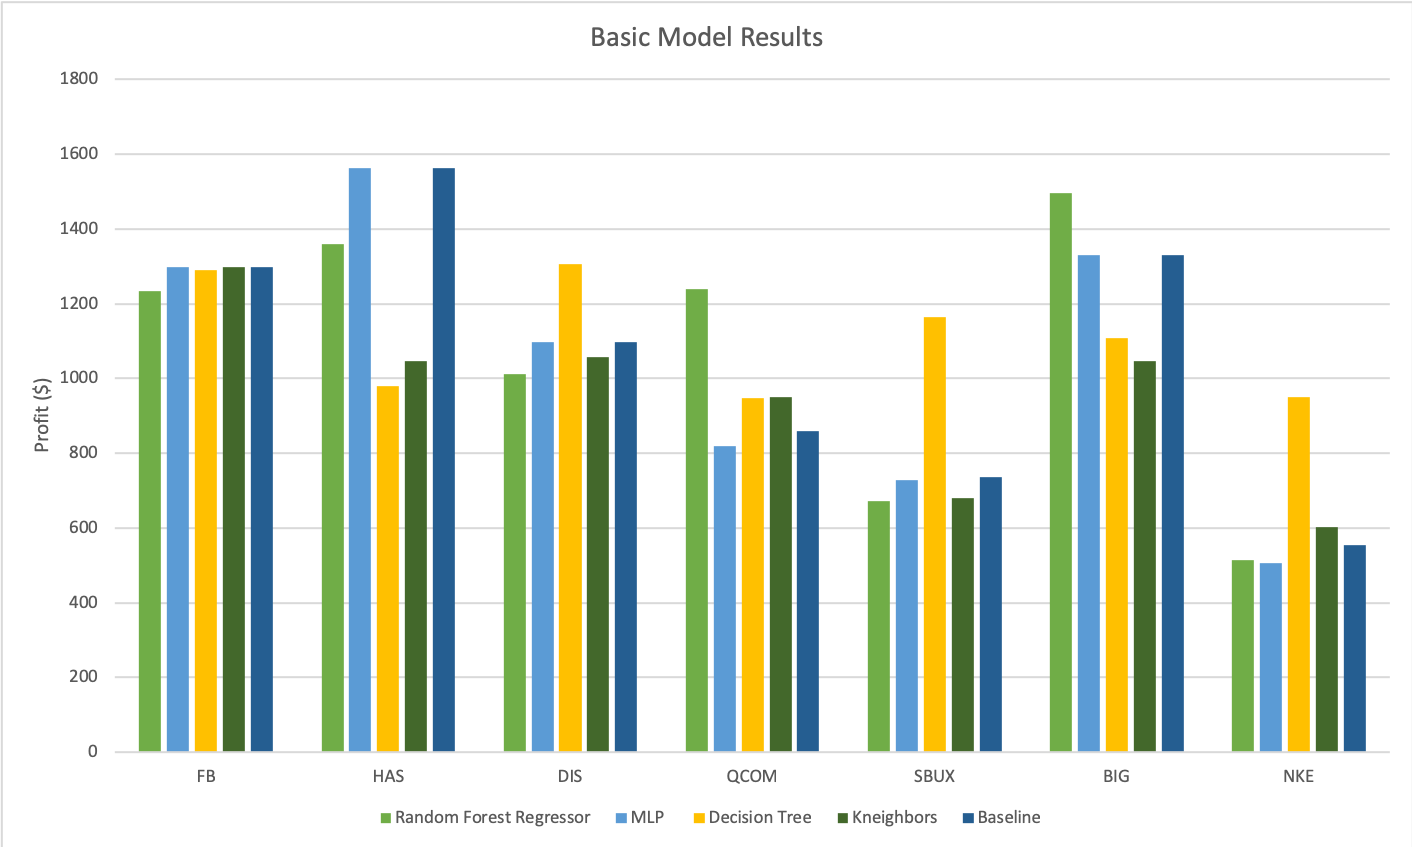
\includegraphics[width=.9\textwidth]{BasicModelResults.png}
\caption{Basic Model Results \label{overflow}}
\label{simpleresults}
\end{figure}

\section{Extended Model}
Our extended model that adds additional twitter features for the input has an overall improvement over the basic model that only takes in closing price and twitter sentiment. Figure~\ref{complexresults} shows the performance of a selection of stocks that were tested. We find that 82.4\% of the stocks tested have a particular algorithm that beats the baseline. This is an improvement of 53\% moving to a model with more inputs. This means that including features such as amount of tweets and retweets are useful for stock trading. Specifically, AMD has the most remarkable performance, with the decision tree classifier generating 629.1\% profit and doubling the baseline profit. We find MNST to also have impressive returns with this model. the decision tree classifier generates a 79\% profit while the baseline nets a loss of 31.2\%. The random forest regressor of BIG generates 88.7\% profit, beating the baseline by 55.7\%. These returns for specific models on specific stocks are significant enough to implement for a realtime for-profit trading algorithm, showing that twitter sentiment can be used to aid stock trading.

\begin{figure}[h]
\centering
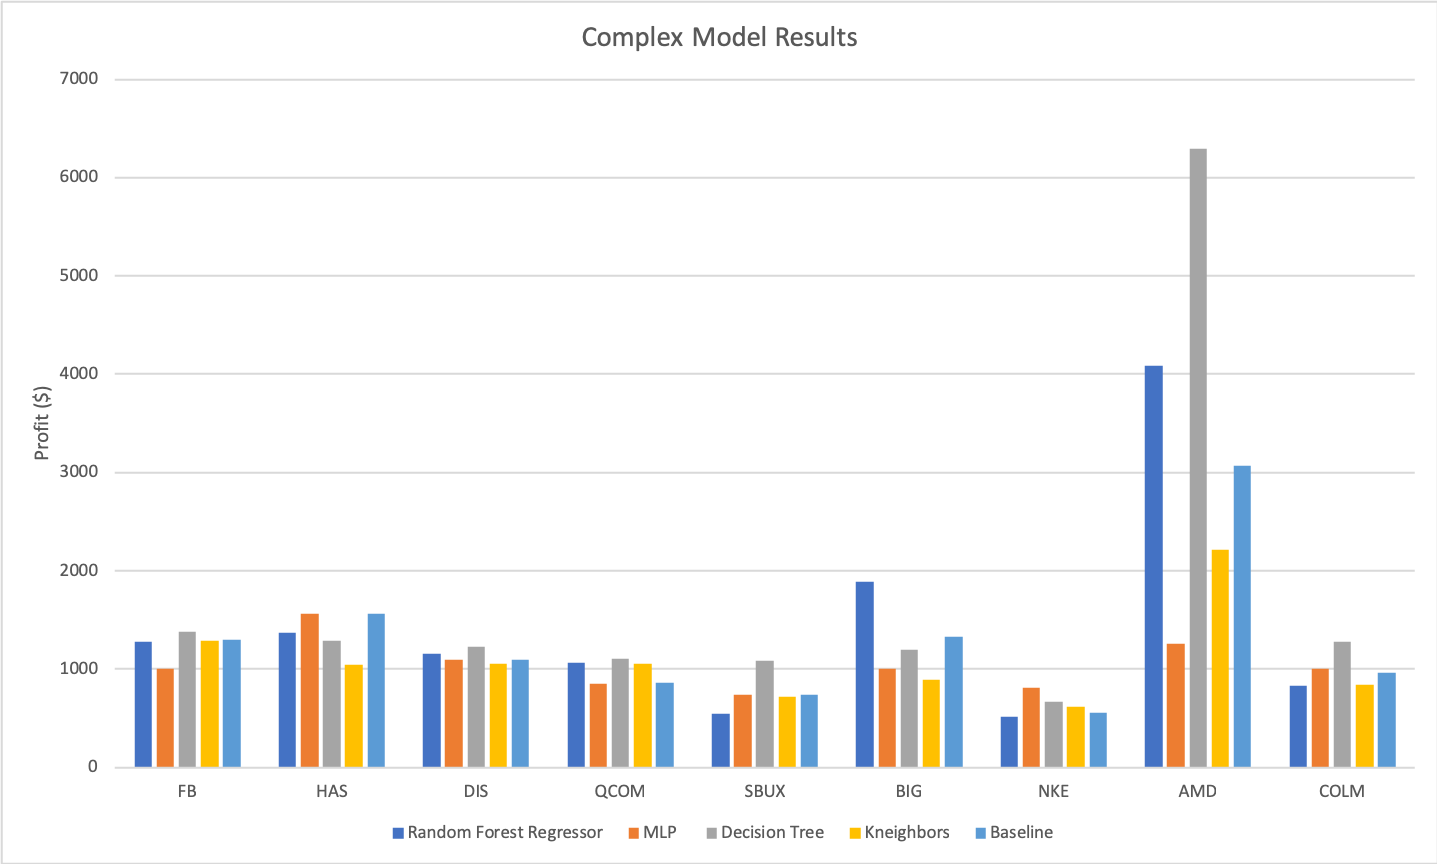
\includegraphics[width=.9\textwidth]{ComplexModelResults.png}
\caption{Extended Model Results \label{overflow}}
\label{complexresults}
\end{figure}

\section{Stacking Model}
Our stacking model that aggregates all of our various machine learning models into one buy or sell signal doesn't perform as well as the extended model, but handily beats the basic model. Figure~\ref{complexresults} shows the performance of a selection of stocks that were tested. We find that 58.8\% of the stocks using the conservative strategy beat the baseline, while only 29.4\% of the lenient strategy beat the baseline. In particular, MNST has fantastic performance, netting a 50\% profit while the baseline nets a loss of 23.7\% while using the lenient strategy. EBAY's conservative strategy has a 6.9\% return while the baseline has a 39.5\% loss. In these results, the stocks that end up beating the baseline are generally because of the baseline losing money over the trading period. While a few stocks do end up beating a high performing baseline, this strategy like others using twitter sentiment, performs much better when the stock does poorly over the trading period. 

\begin{figure}[h]
\centering
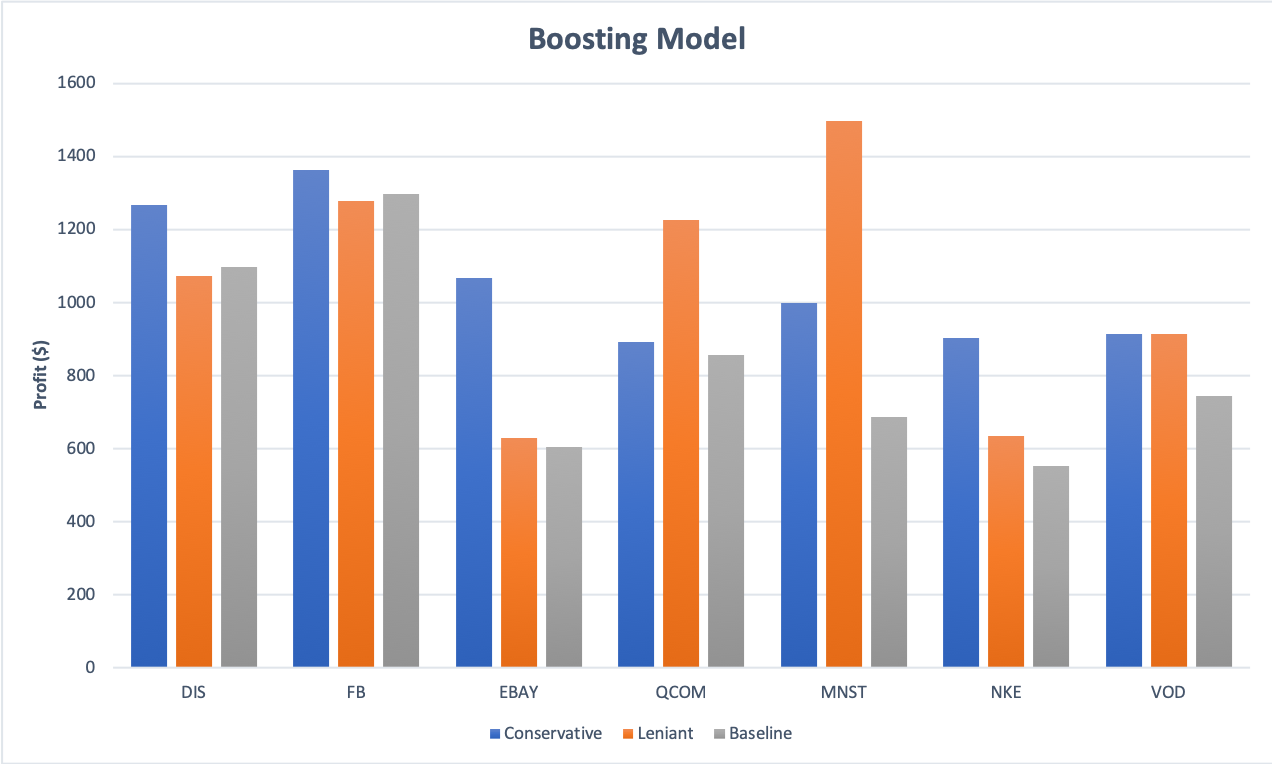
\includegraphics[width=.9\textwidth]{BoostingModelResults.png}
\caption{Stacking Model Results \label{overflow}}
\label{stackingresults}
\end{figure}

\section{Deep Learning Model}
Our deep learning model acts differently than any of the above models, as it predicts the price of the following days close. This model has more average performance, but is far more consistent. Rarely does a particular stock trading on the strategy truly perform terribly. Figure~\ref{deepresults} shows our results for some specific stocks within the data. The first 5 stocks in the model, QCOM to MSFT, demonstrate how the strategy hovers close to the baseline and gives consistent performance. Interestingly the last two stocks, EBAY and SBUX, have incredible performance. There is a respective improvement of \$559.53 and \$785.71 for our strategy over the baseline. Given that the initial capital is \$1000, these are some truly astonishing results. 


While we do find far less instances of beating the baseline, our model has far more consistent performance than any of the others discussed above. This is most likely attributed to the accuracy of the predicted stock prices. The RMSE of all of our stocks range between 1.5 and 2.5, signifying that our model is able to predict the closing price of stocks extremely closely. While the predicted price is close, it isn't accurate enough to be consistently profitable. This performance is most likely due the model predicting stock prices for multiple days in a row either above or below the current price, which hampers performance for our end-of-day trading strategy that is entirely reliant on  predictions of price change up or down. Future work could predict multiple days of stock prices in the future and then act on sustained performance rather than specific day-by-day changes to help with this issue in our strategy. 

\begin{figure}[h]
\centering
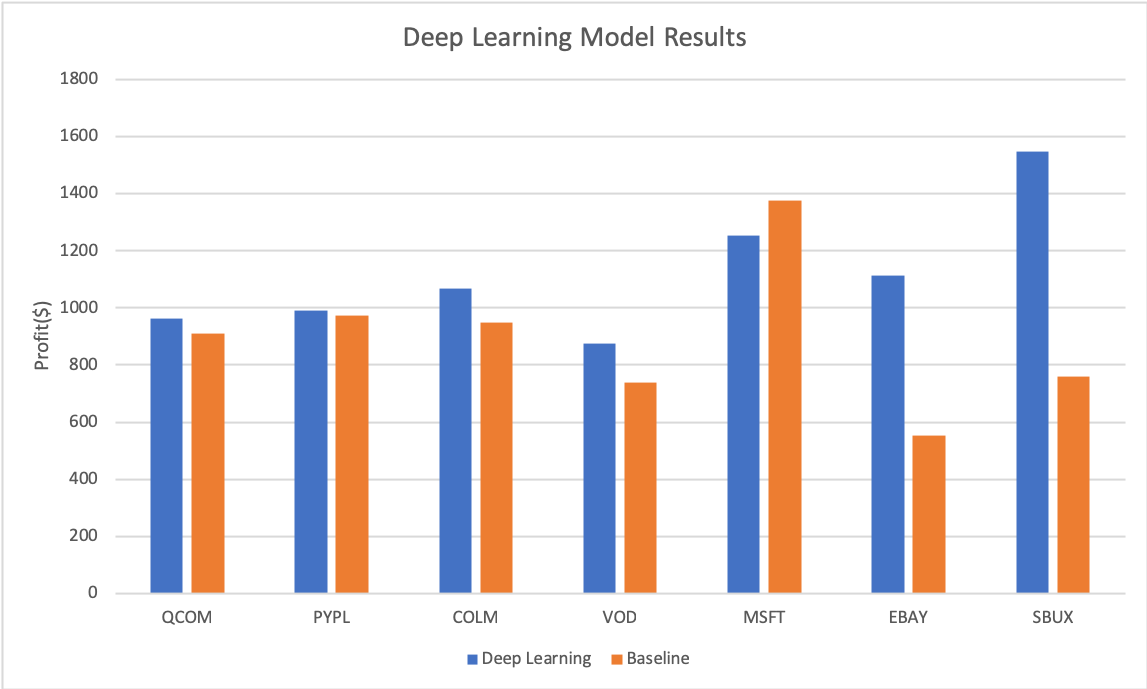
\includegraphics[width=.9\textwidth]{DeepLearningResults.png}
\caption{Deep Learning Model Results \label{overflow}}
\label{deepresults}
\end{figure}

\end{document}
